% Provenance (never printed): see sources/outline_sources.md (Year 3:
% geomorphology, hillslope processes, river incision, landscape evolution).
% Brief: sources/book5/BRIEFS.md, ch. 18. Curves from
% figdata/bachelor-3/hillslope.py, stream_profile.py and varden_river.py.
% Exercise and problem values in the Book 5 scratch calculator calc/ch18.py.
% The upland west of the Varden Hills, its river, its tributaries, its
% uplift rate and its base-level fall are invented; the outlet elevation is
% the region model's river at the west edge of the map.
\chapter{الجيومورفولوجيا الكمّية}\label{ch:b3:quantitative-geomorphology}

يعبر نهرٌ سلسلةً جبليةً صاعدةً، فيكون لمقطعه الطولي درجةٌ: شلالٌ،
يقع أسفله مضيقٌ، ويمتدّ أعلاه واديٌ أقلّ انحدارًا. لا تبقى الدرجةُ
حيث تكوّنت، بل تصعد نحو المنبع بمقدار بضعة ملّيمترات أو بضعة أمتار في
السنة، ويمثّل موضعها ساعةً بدأت حين انخفض مستوى قاعدة النهر.
وقراءة تلك الساعة، والمعدّلات المكتوبة في أشكال التلال والأنهار، تتطلّب
قانونَي حفظٍ وقانونَي نقلٍ: أحدهما للتربة التي تزحف نزولًا على المنحدر،
والآخر للصخر الأساسي الذي يقطعه النهر.

\begin{recall}
التجوية والتعرية والترسيب والأشكال الأرضية والتوازن بين الرفع والتعرية
واردةٌ في كتب المدرسة، وكذلك الارتداد الأيزوستاتي والأودية الجليدية ذات
المقطع على شكل حرف U. ويرد معدّل التجريد وإجهاد القصّ القاعي ومعامل شيلدز
في مجلد السنة الأولى، في فصله عن التعرية والنقل؛
ونموذج الارتفاع الرقمي في فصله عن الخرائط الجيولوجية؛ وتوازن إيري
في فصله عن التوازن الأيزوستاتي وشذوذات الجاذبية. وترد النويدات الكونية المنشأ
ومعدّلات التعرية المستمدّة منها في
الفصل~\ref{ch:b3:advanced-geochronology}، \omterm{def:b3:orogenic-wedges:thermochronology}{والكرونولوجيا الحرارية} \omterm{def:b3:orogenic-wedges:age-elevation}{وعلاقة
العمر بالارتفاع} في الفصل~\ref{ch:b3:orogenic-wedges}. وترد معادلة
الانتشار في كتب الفيزياء.
\end{recall}

\section{السفوح}\label{sec:b3:quantitative-geomorphology:hillslopes}

على تلّةٍ مكسوّةٍ بالتربة تتحرّك التربةُ نحو الأسفل حبّةً حبّةً: تقذفها الحيوانات
الحافرة، وترفعها الجذور، ويوسّعها التجمّد والترطّب، وكلّ
اضطرابٍ يدع الجاذبية تزيحها قليلًا. ومتوسّطًا على مدى القرون،
يتناسب دفق التربة طرديًّا مع الانحدار.

\begin{definition}[انتشار السفوح]\label{def:b3:quantitative-geomorphology:diffusion}
\emph{انتشار السفوح}\index{انتشار السفوح} هو النقل البطيء للتربة نحو الأسفل،
الذي يكون دفقه الحجمي لكلّ وحدة عرض من السفح،
$\vec q$، يتناسب طرديًّا مع تدرّج الارتفاع السطحي $z$:
$\vec q = -\kappa\,\nabla z$. ومعامل $\kappa$، الذي يُقاس بوحدة
\unit{m^2/yr}، هو معامل انتشار السفوح.
\end{definition}

\begin{theorem}[انتشار السفوح]\label{thm:b3:quantitative-geomorphology:diffusion}
لتكن الصخور مرفوعةً بمعدّل $U$ بالنسبة إلى القنوات التي تحدّ
سفحًا، وللتربة والصخر الكثافةُ نفسُها، وتنتقل التربة \omterm{def:b3:quantitative-geomorphology:diffusion}{بانتشار السفوح}
بمعامل $\kappa$ منتظم. عندئذٍ يخضع الارتفاع السطحي للمعادلة الآتية:
\[
\frac{\partial z}{\partial t} = U + \kappa\,\nabla^2 z ,
\]
وهي معادلة الانتشار مع حدّ منبعي.
\end{theorem}

\begin{proof}
نأخذ مساحةً صغيرةً $\delta S$ من السفح. يتغيّر حجمها بالرفع،
$U\,\delta S$ في وحدة الزمن، وبالتربة التي تخرج من
حوافّها، $\oint \vec q\cdot\vec n\,\mathrm{d}\ell = (\nabla\cdot\vec q)\,\delta S$.
ومنه $\partial z/\partial t = U - \nabla\cdot\vec q$؛ وبوضع $\vec q = -\kappa
\nabla z$ و$\kappa$ منتظمٌ، $\nabla\cdot\vec q = -\kappa\nabla^2 z$.
\end{proof}

يُنشئ الصدعُ أو خطُّ الشاطئ الجرفَ الصدعيَّ في لحظةٍ واحدةٍ؛ وبعد ذلك
ينتشر الجرف الصدعي فقط. ابتداءً من خطوة رأسية بنصف ارتفاع $a$ على
سفح بعيد بميل $b$، يكون الحلّ في بُعد واحد هو
\[
z(x,t) = a\,\operatorname{erf}\!\left(\frac{x}{2\sqrt{\kappa t}}\right) + b\,x ,
\qquad
\left.\frac{\partial z}{\partial x}\right|_{x=0} = \frac{a}{\sqrt{\pi\kappa t}} + b .
\]
يعتمد الشكل على الجداء $\kappa t$ وحده: يعطي المقطعُ المقيسُ
$\kappa t$، فإمّا أن يعطي عمرٌ مستقلٌّ $\kappa$، وإمّا أن يعطي
$\kappa$ المعلوم العمرَ، وهو \emph{العمر المورفولوجي}. تعطي الجروف الصدعية في المناطق
شبه الجافة ذات التربة الحبيبية والغطاء النباتي المتفرّق قيمة $\kappa$ بين
$10^{-3}$ و\qty{e-2}{m^2/yr}؛ أمّا الجبال الساحلية الرطبة الكثيفة الغطاء النباتي
فتبلغ نحو \qty{5e-3}{m^2/yr}.
% ledger: whipple04:scarp-erf, whipple04:scarp-kappa

\begin{omfigure}
\begin{tikzpicture}
\begin{groupplot}[group style={group size=2 by 1, horizontal sep=1.6cm},
  width=0.48\linewidth, height=0.36\linewidth, tick label style={font=\scriptsize},
  label style={font=\small}, legend style={font=\scriptsize, draw=none, fill=none}]
\nextgroupplot[xlabel={المسافة $x$ \babelsublr{(m)}}, ylabel={الارتفاع $z$ \babelsublr{(m)}}, xmin=-40, xmax=40,
  ymin=-5, ymax=5, legend pos=north west]
% computed in figdata/bachelor-3/hillslope.py
\addplot[black!50, densely dashed] table[x=x, y=z0] {figdata/out/bachelor-3-hillslope-scarp.dat};
\addplot[omDef, thick] table[x=x, y=z1] {figdata/out/bachelor-3-hillslope-scarp.dat};
\addplot[omProp, thick] table[x=x, y=z2] {figdata/out/bachelor-3-hillslope-scarp.dat};
\addplot[omThm, thick] table[x=x, y=z3] {figdata/out/bachelor-3-hillslope-scarp.dat};
\legend{{الابتدائي}, \qty{2}{kyr}, \qty{10}{kyr}, \qty{40}{kyr}}
\nextgroupplot[xlabel={المسافة من خطّ التقسيم \babelsublr{(m)}}, ylabel={الارتفاع \babelsublr{(m)}},
  xmin=-150, xmax=150, ymin=0, ymax=200, xtick={-150,-75,0,75,150}]
\addplot[omMeth, thick] table[x=x, y=z1] {figdata/out/bachelor-3-hillslope-hill.dat};
\addplot[omDef, thick] table[x=x, y=z2] {figdata/out/bachelor-3-hillslope-hill.dat};
\addplot[omThm, thick] table[x=x, y=z3] {figdata/out/bachelor-3-hillslope-hill.dat};
\node[font=\scriptsize, anchor=north] at (axis cs:0,45) {0.0215};
\node[font=\scriptsize, anchor=north] at (axis cs:0,94) {0.043};
\node[font=\scriptsize, anchor=north] at (axis cs:0,184) {\qty{0.086}{mm/yr}};
\end{groupplot}
\end{tikzpicture}

\par\smallskip{\small يسارًا، جرفٌ صدعيّ بإزاحة \qty{5}{m} على سفح ميله
0.05، ينتشر بمعامل $\kappa = \qty{5e-3}{m^2/yr}$: الخطوةُ الابتدائيةُ
(المتقطّعة) والمقاطعُ بعد 2 و10 و\qty{40}{kyr}. يمينًا، تلالٌ
مستقرّة بنصف عرض \qty{150}{m} وبالمعامل $\kappa$ نفسه (الارتفاع فوق
القنوات)، تنخفض بمعدّلات
0.0215 و0.043 و\qty{0.086}{mm/yr}: قطوعٌ مكافئةٌ يتناسب فيها ارتفاع التضاريس
وانحناء القمم طرديًّا مع معدّل التعرية.}\label{fig:b3:quantitative-geomorphology:hillslope}
\end{omfigure}
% ledger: whipple04:scarp-kappa

إذا رُفعت تلّةٌ وتعرّضت للتعرية زمنًا كافيًا، توقّف شكلها عن
التغيّر: يتناقص ارتفاع كلّ نقطةٍ بالمعدّل نفسه الذي يرتفع به الصخر.

\begin{proposition}[انحناء القمّة يقيس معدّل التعرية]\label{prop:b3:quantitative-geomorphology:curvature}
على سفحٍ في \omterm{def:b3:quantitative-geomorphology:steady-profile}{الحالة المستقرّة} تحت \omterm{def:b3:quantitative-geomorphology:diffusion}{انتشار السفوح}، يكون معدّل التعرية
$E$ الذي يساوي $U$ هو
\[
E = -\kappa\,\nabla^2 z .
\]
في بُعدٍ واحد يكون المقطع الطولي هو القطعَ المكافئ $z = z_0 - E x^2/(2\kappa)$،
مع تضاريسَ قدرها $E L^2/(2\kappa)$ بين خطّ التقسيم والقنوات التي تبعد مسافةً
$L$ عن خطّ التقسيم.
\end{proposition}

\begin{proof}
بوضع $\partial z/\partial t = 0$ في المبرهنة نحصل على $\kappa\nabla^2 z =
-U = -E$. في بُعدٍ واحد، يعطي تكامُلان مع $\mathrm{d}z/\mathrm{d}x =
0$ عند خطّ التقسيم القطعَ المكافئ، وقيمتُه عند $x = L$ هي التضاريس.
\end{proof}

ومنه، فإنّ الانحناء، وهو كمّيةٌ هندسيّةٌ تُقاس على نموذج الارتفاع الرقمي،
يُقرأ معدّلًا بمجرّد معرفة $\kappa$: فكلّما كانت قمم التلال أشدّ انحدارًا وأكثر استدارةً،
تسارعت تعرّي المشهد. وتتكوّن التربة نفسها من الصخر الذي تحتها
بمعدّلٍ يتوقّف على مقدار التربة التي تغطّيه أصلًا.

\begin{definition}[دالة إنتاج التربة]\label{def:b3:quantitative-geomorphology:soil-production}
\emph{دالة إنتاج التربة}\index{دالة إنتاج التربة} تعطي
المعدّل $P$ الذي يتحوّل عنده الصخر الأساسي إلى تربة بوصفه دالةً في سماكة التربة
$h$؛ وتُؤخذ عادةً على الصورة $P = P_0\,e^{-h/h_0}$، حيث
$P_0$ هو المعدّل على الصخر العاري، و$h_0$ طولٌ يبلغ جزءًا من المتر.
\end{definition}

عند \omterm{def:b3:quantitative-geomorphology:steady-profile}{الحالة المستقرّة} يهبط السطح الفاصل بين التربة والصخر بمعدّل
السطح، أي $P(h) = E$، فتكون سماكة التربة $h = h_0 \ln(P_0/E)$: كلّما كانت التعرية أسرع كانت التربة أرقّ،
وحيث يتجاوز $E$ القيمة $P_0$ تُجرَّد التربة
ويظهر الصخر العاري المحدود بالتجوية. أسرع معدّلات إنتاج التربة
المقاسة من مرتبة \qty{0.5}{mm/yr}.
% ledger: whipple04:soil

تُخفق الانتشاريّة الخطيّة على المنحدرات الشديدة. فمع اقتراب الانحدار من
عتبةٍ معيّنة، تتدحرج الحبيبات وتنزلق على شكل دفعات، وتجرّد الانزلاقاتُ الأرضيّة الضحلة
التربةَ.

\begin{definition}[انحدار السفح الحرج]\label{def:b3:quantitative-geomorphology:critical}
\emph{انحدار السفح الحرج}\index{انحدار السفح الحرج}
$S_c$ هو الانحدار الذي يتزايد عنده دفق التربة دون حدّ؛ وفي
قانون نقلٍ غير خطّيّ شائع الاستعمال، $q = \kappa S/[1 - (S/S_c)^2]$.
\end{definition}

تتصرّف المنحدرات الأقلّ انحدارًا بكثير من $S_c$ كما في الانتشاريّة الخطيّة؛ أمّا المنحدرات
التي تتعرّى بسرعة فتزداد انحدارًا نحو $S_c$ وتصير مستوية، ويُضبط انحدارها
بالعتبة لا بمعدّل التعرية.
% ledger: whipple04:nonlinear

\begin{inthefield}[مسح سفحٍ]
يضع فريقٌ يمسح حافةً تكسوها التربة جهازَ مسحٍ ليزريًّا أرضيًّا على حامل ثلاثيّ
على بُعد بضعة عشرات الأمتار من القمّة. يسجّل كلّ مسحٍ ملايينَ النقاط،
أي المسافةَ والاتجاهَ إلى سطح الأرض عبر الفجوات
بين الحشائش والشجيرات؛ وتُدمج نقاطُ عدّة محطّات مسحٍ
في سحابةٍ واحدة، تُطابَق على أهدافٍ مُساحةٍ بمستقبِل الأقمار الصناعية،
وتُحفظ آخر الانعكاسات لإزالة الغطاء النباتي. وتُحوَّل سحابة الأرض المكشوفة
إلى شبكةٍ من نموذج الارتفاع بخلايا بحجم ديسيمتر، تُنعَّم على مسافة بضعة
أمتار، ويُحسب لابلاسيانها عند القمّة. ثم يقارن الفريق انحناءات
قمم الحواف التي تتعرّى بمعدّلات قيسَت بالنويدات الكونية
المنشأ؛ وعند رسم الكميّتين إحداهما مقابل الأخرى، تعطيان معامل الانتشار
للسفح بوصفه ميلَ الخطّ المستقيم، كما تتنبّأ القضية.
\end{inthefield}

\section{الحفر النهري}\label{sec:b3:quantitative-geomorphology:rivers}

حيث يجري النهر على صخرٍ أساسيّ، يقطع الصخرَ إلى أسفل بانتزاع الكتل،
وبالتآكل بفعل حمولة القاع، وبالتكهّف. وتتناسب هذه الآليات كلّها مع إجهاد القصّ
الذي يمارسه التيّار على قاعه، أو مع الاستطاعة التي يبذلها هناك،
وتزداد كلتاهما مع التصريف والانحدار. ويزداد التصريف مع مساحة الحوض الصبّي،
فتقوم المساحة مقام التصريف.

\begin{definition}[قانون قدرة المجرى]\label{def:b3:quantitative-geomorphology:stream-power}
\emph{قانون قدرة المجرى}\index{قانون قدرة المجرى} يعطي معدّل الحفر الرأسي $E$ لنهرٍ على صخرٍ أساسيّ
على الصورة
\[
E = K A^m S^n ,
\]
حيث $A$ هي مساحة الحوض الصبّي عند النقطة، و$S$ انحدار القناة،
و$m$ و$n$ أُسّان موجبان، و$K$ معامل القابلية للتعرية
الذي يجمع قوّة الصخر والمناخ وعرض القناة.
\end{definition}

بالنسبة إلى العمليات التي تتناسب مع إجهاد القصّ أو مع استطاعة التيّار الوحدوية،
تكون النسبة $m/n$ قريبةً من 0.5. وقد وجد مسحٌ لقنوات الأراضي الوعرة المحفورة في صخرٍ ضعيف
على مدى نحو 20 عامًا أنّ معدّلات الحفر تتناسب مع $A^{0.44}S^{0.68}$.
% ledger: whipple04:spim

\begin{definition}[الحفر المحدود بالاقتلاع والمحدود بالنقل]\label{def:b3:quantitative-geomorphology:limited}
يكون الحفر \emph{محدودًا بالاقتلاع}\index{محدودًا بالاقتلاع}
حين يستطيع النهر حمل رواسبَ أكثر مما يتلقّاه، بحيث يُضبط معدّل خفضه
بمدى سرعة اقتلاع النهر للصخر الأساسي من قاعه:
وهنا يسري \omterm{def:b3:quantitative-geomorphology:stream-power}{قانون قدرة المجرى}. ويكون
\emph{محدودًا بالنقل}\index{محدودًا بالنقل} حين يحمل النهر
كلّ الرواسب التي يستطيع حملها، فلا يُخفَض قاعه إلّا حيث
تزداد قدرة النقل باتّجاه المصبّ، وبالمعدّل الذي يضبطه تباعد
دفق الرواسب.
\end{definition}

يتصرّف النهر \omterm{def:b3:quantitative-geomorphology:limited}{المحدود بالنقل} تصرّفًا قريبًا من السفح: يتعلّق الدفق بالانحدار،
ويتطوّر مقطعه الطولي وفق معادلة شبيهة بالانتشار تُسوّي أيّ درجةٍ صغيرة.
أمّا النهر \omterm{def:b3:quantitative-geomorphology:limited}{المحدود بالاقتلاع} فيُبقي الدرجة حادّة ويُزيحها،
كما يُبيّن القسم التالي. وتكون أنهار الجبال ذات القيعان الصخرية والحصى الرقيق
أقرب عادةً إلى النوع الأول،
والأنهار الجارية على رواسب فيضيّة سميكة إلى النوع الثاني.

\begin{omfigure}
\begin{tikzpicture}[x=0.55cm, y=0.55cm, font=\scriptsize,
  declare function={f(\x)=2.1+3.5*(1-(\x-0.5)/10)^2;
    tl(\x,\l)=f(\x)-1.1*exp(-(10.5-\x)/\l);}]
\begin{scope}
\draw[->] (0,0) -- (11.5,0) node[below left] {المسافة باتجاه المصبّ};
\draw[->] (0,0) -- (0,6) node[above right] {$z$};
\draw[black!50, densely dashed] plot[domain=0.5:10.5, samples=40] (\x,{f(\x)});
\draw[omDef, thick] plot[domain=0.5:6.5, samples=30] (\x,{f(\x)}) -- plot[domain=6.5:10.5, samples=20] (\x,{f(\x)-1.1});
\draw[omThm, thick] plot[domain=0.5:3.5, samples=20] (\x,{f(\x)}) -- plot[domain=3.5:10.5, samples=30] (\x,{f(\x)-1.1});
\draw[->, black!70] (6.3,4.1) -- (3.8,4.75);
\node[anchor=west, align=left] at (5.6,5.3) {\foreignlanguage{arabic}{محدود بالاقتلاع:}\\ الخطوة تتحرّك نحو المنبع};
\node at (5.5,-0.7) {(أ)};
\end{scope}
\begin{scope}[xshift=7.2cm]
\draw[->] (0,0) -- (11.5,0) node[below left] {المسافة باتجاه المصبّ};
\draw[->] (0,0) -- (0,6) node[above right] {$z$};
\draw[black!50, densely dashed] plot[domain=0.5:10.5, samples=40] (\x,{f(\x)});
\draw[omDef, thick] plot[domain=0.5:10.5, samples=40] (\x,{tl(\x,1.2)});
\draw[omThm, thick] plot[domain=0.5:10.5, samples=40] (\x,{tl(\x,3.5)});
\node[anchor=west, align=left] at (5.0,5.3) {\foreignlanguage{arabic}{محدود بالنقل:}\\ الهبوط ينتشر نحو المنبع};
\node at (5.5,-0.7) {(ب)};
\end{scope}
\end{tikzpicture}

\par\smallskip{\small استجابة النهر لهبوط مستوى قاعدته
(المتقطّع: المقطع قبل الهبوط؛ الأزرق ثم الأحمر: لحظتان لاحقتان)،
رسم تخطيطي. (أ) النهر \omterm{def:b3:quantitative-geomorphology:limited}{المحدود بالاقتلاع} يحتفظ بنقطة انقطاع حادّة تتحرّك
نحو المنبع؛ وتحتها يحتفظ المقطع بشكله القديم، لكنه منخفض. (ب) النهر \omterm{def:b3:quantitative-geomorphology:limited}{المحدود
بالنقل} يخفض مقطعه كلّه تدريجيًا، وأكثر ما يكون ذلك قرب
المصبّ.}\label{fig:b3:quantitative-geomorphology:regimes}
\end{omfigure}

إذا ارتفع الصخر بمعدّل ثابت $U$ بالنسبة إلى مصبّ النهر، و$K$،
$m$، $n$ ثوابت، يتطوّر النهر وفق $\partial z/\partial t = U - K A^m
S^n$.

\begin{definition}[مقطع النهر في الحالة المستقرّة]\label{def:b3:quantitative-geomorphology:steady-profile}
يكون مقطع النهر في \emph{الحالة المستقرّة}\index{مقطع النهر في الحالة المستقرّة}
عندما لا يتغيّر ارتفاعه مع الزمن: عند كلّ نقطة يوازن الحفرُ
رفعَ الصخر بالنسبة إلى المصبّ.
\end{definition}

\begin{theorem}[المقطع في الحالة المستقرّة وفق قانون قدرة المجرى]\label{thm:b3:quantitative-geomorphology:steady}
عند ثبات $U$، $K$، $m$ و$n$، يملك النهر \omterm{def:b3:quantitative-geomorphology:limited}{المحدود بالاقتلاع} في
\omterm{def:b3:quantitative-geomorphology:steady-profile}{الحالة المستقرّة} الانحدار
\[
S = \left(\frac{U}{K}\right)^{1/n} A^{-m/n} .
\]
\end{theorem}

\begin{proof}
في \omterm{def:b3:quantitative-geomorphology:steady-profile}{الحالة المستقرّة} $\partial z/\partial t = 0$، إذن $K A^m S^n = U$، ومنه $S^n
= (U/K)A^{-m}$؛ بأخذ الجذر من الدرجة $n$ نحصل على النتيجة.
\end{proof}

\begin{omfigure}
\begin{tikzpicture}
\begin{groupplot}[group style={group size=2 by 1, horizontal sep=1.7cm},
  width=0.48\linewidth, height=0.33\linewidth, tick label style={font=\scriptsize},
  label style={font=\small}]
\nextgroupplot[xlabel={المسافة من خطّ تقسيم المياه \babelsublr{(\unit{km})}}, ylabel={\mbox{\textdir TLT $z$ (\unit{m})}},
  xmin=0, xmax=12, ymin=150, ymax=420]
% computed in figdata/bachelor-3/stream_profile.py
\addplot[omDef, thick] table[x=d, y=z] {figdata/out/bachelor-3-stream_profile-steady.dat};
\nextgroupplot[xmode=log, ymode=log, xlabel={مساحة التصريف $A$ \babelsublr{(\unit{km^2})}},
  ylabel={الانحدار $S$}, xmin=0.1, xmax=100, ymin=0.003, ymax=0.2]
\addplot[omDef, thick] table[x=A, y=S] {figdata/out/bachelor-3-stream_profile-steady.dat};
\addplot[only marks, mark=*, mark size=1.4pt, omThm] table[x=A, y=S] {figdata/out/bachelor-3-stream_profile-sa.dat};
\addplot[omThm, densely dashed] table[x=A, y=S] {figdata/out/bachelor-3-stream_profile-fit.dat};
\end{groupplot}
\end{tikzpicture}

\par\smallskip{\small المقطع في \omterm{def:b3:quantitative-geomorphology:steady-profile}{الحالة المستقرّة} للنهر المتخيّل في المرتفعات
الواقع غرب تلال فاردن ($U = \qty{0.043}{mm/yr}$، $K =
\qty{e-6}{yr^{-1}}$، $m = 0.5$، $n = 1$)، من رأس القناة إلى
المصبّ عند \qty{170}{m}. يمينًا: الانحدار مقابل المساحة: النموذج (الخطّ الأزرق)
واثنا عشر انحدارًا مقيسًا على مقاطع طول كلّ منها \qty{200}{m} بتشتّت
نحو \qty{10}{\percent} (النقاط الحمراء)، وخطّ المربعات الصغرى
(المتقطّع) ميله $-0.47$.}\label{fig:b3:quantitative-geomorphology:profile}
\end{omfigure}

ينخفض الانحدار بوصفه قوّةً للمساحة: المقطع مقعّر نحو الأعلى. والأنهار الحقيقية
تتّبع قانون القوّة هذا حتى حين تكون افتراضات المبرهنة
موضع شكّ، فيكفي عددان لتلخيص المقطع.
% ledger: whipple04:steepness

\begin{definition}[مؤشّرا انحدار القناة والتقعّر]\label{def:b3:quantitative-geomorphology:indices}
عندما يتبع انحدار النهر $S = k_s A^{-\theta}$، يُسمّى الأسّ
$\theta$ هو \emph{مؤشّر التقعّر}\index{مؤشّر التقعّر}، والمعامل
$k_s$ هو \emph{مؤشّر انحدار القناة}\index{مؤشّر انحدار القناة}.
ولمقارنة الأنهار يُضبط $\theta$ على قيمة مرجعية مشتركة
$\theta_{\mathrm{ref}}$، و$k_{sn} = S A^{\theta_{\mathrm{ref}}}$ هو
الانحدار المعيّر.
\end{definition}

وبحسب المبرهنة، $\theta = m/n$ و$k_s = (U/K)^{1/n}$: عند قابلية تعرية معيّنة،
يكون النهر أشدّ انحدارًا حيث يرتفع الصخر أسرع. وخرائط الانحدار
لسلسلة جبلية تُظهر بذلك ملامح رفعها.


الانحدارات مشتقّات لارتفاعات مشوبة بالضجيج، وتتشتّت تشتّتًا واسعًا. أمّا
تكامل المقطع فيستخدم الارتفاعات، وهي أفضل قياسًا.

\begin{definition}[تحليل كاي]\label{def:b3:quantitative-geomorphology:chi}
\emph{تحليل كاي}\index{تحليل كاي} يرسم ارتفاع نقاط
شبكة نهرية مقابل الإحداثيّ
\[
\chi(x) = \int_{x_b}^{x} \left(\frac{A_0}{A(x')}\right)^{\theta}
\mathrm{d}x' ,
\]
حيث $x$ هي المسافة نحو المنبع على طول القناة، انطلاقًا من نقطة الأساس
$x_b$، و$A_0$ مساحة مرجعية، و$\theta$ \omterm{def:b3:quantitative-geomorphology:indices}{مؤشّر التقعّر}؛ و$\chi$ له
بُعد الطول.
\end{definition}

\begin{proposition}[تحوّل كاي يُقوّم القطع الطولي المستقرّ]\label{prop:b3:quantitative-geomorphology:chi}
تحت افتراضات مبرهنة \omterm{def:b3:quantitative-geomorphology:steady-profile}{الحالة المستقرّة}، مع $\theta = m/n$،
كل قناة في شبكة تصرّف إلى منسوب القاعدة $z_b$ تحقّق
\[
z = z_b + \left(\frac{U}{K A_0^{m}}\right)^{1/n} \chi :
\]
تقع كل القنوات على خطّ مستقيم واحد ميله $k_s A_0^{-\theta}$ في
المستوي $(\chi, z)$.
\end{proposition}

\begin{proof}
على طول القناة، $\mathrm{d}z/\mathrm{d}x = S = k_s A^{-\theta} = k_s
A_0^{-\theta}(A_0/A)^{\theta}$. بالتكامل انطلاقًا من $x_b$، حيث $z = z_b$،
نجد $z = z_b + k_s A_0^{-\theta}\chi$، و$k_s A_0^{-\theta} =
(U/K)^{1/n} A_0^{-m/n}$. يصبّ الرافد في الجذع عند نقطة وصل يتشارك عندها
قيمتي $z$ و$\chi$ معه، ويخضع للعلاقة نفسها نحو المنبع منها.
\end{proof}

القناة التي تنحرف عن الخطّ ليست في حالة مستقرّة، أو تعبر
صخرًا ذا قابلية تعرية مختلفة، أو فقدت مساحة تصريف أو اكتسبتها:
الرافد الذي يقع فوق جيرانه عند القيمة نفسها من $\chi$ يُسلب مساحته،
والرافد الذي يقع أسفلها ينمو.

\section{التضاريس الانتقالية}\label{sec:b3:quantitative-geomorphology:transient}

\begin{definition}[مستوى القاعدة ونقطة الانقطاع]\label{def:b3:quantitative-geomorphology:knickpoint}
\emph{مستوى القاعدة}\index{مستوى القاعدة} لنهر هو منسوب مصبّه،
الذي لا يستطيع النهر الحفر دونه: البحر، أو بحيرة، أو النهر الرئيسي الذي
يصبّ فيه. \emph{نقطة الانقطاع}\index{نقطة الانقطاع} موضع يتزايد فيه انحدار
المقطع الطولي للنهر فجأةً، من مقطع مُنحدِر إلى
شلّال.
\end{definition}

قد تكون \omterm{def:b3:quantitative-geomorphology:knickpoint}{نقطة الانقطاع} ثابتة، حيث يعبر النهر قاعًا أصلب أو
جرفًا صدعيًا ما زال نشطًا، أو متحرّكة، حيث تمثّل رأس
استجابة النهر لتغيّر يقع أسفلها: انخفاض \omterm{def:b3:quantitative-geomorphology:knickpoint}{مستوى القاعدة}، أو
رفعٌ أسرع.
% ledger: whipple04:response

\begin{theorem}[نقاط الانقطاع موجات حركية]\label{thm:b3:quantitative-geomorphology:kinematic}
ليكن $n = 1$، مع ثبات $U$ و$K$ و$m$، وليكن $x$ المسافة
نحو المنبع من المصبّ. عندئذٍ يخضع $z$
\[
\frac{\partial z}{\partial t} + K A^m \frac{\partial z}{\partial x} = U ,
\]
وأيّ ملمح في المقطع، بما فيه الدرجة، ينتقل نحو المنبع بالسرعة
$c = K A^m$ محتفظًا بارتفاعه. نقطة انقطاع تبدأ من
المصبّ عند $t = 0$ تصل إلى النقطة $x$ في الزمن
\[
t(x) = \int_0^x \frac{\mathrm{d}x'}{K A(x')^m} = \frac{\chi(x)}{K A_0^m},
\]
مع حساب $\chi$ عند $\theta = m$. تقع جميع نقاط الانقطاع التي تنشأ في شبكة
في الزمن نفسه إذن عند القيمة نفسها من $\chi$، وعلى الكنتور نفسه.
\end{theorem}

\begin{proof}
مع اعتبار $x$ نحو المنبع، الانحدار هو $S = \partial z/\partial x$،
ومعادلة التطوّر $\partial z/\partial t = U - K A^m S$ هي المعادلة
المكتوبة. على منحنًى $\mathrm{d}x/\mathrm{d}t = K A(x)^m$، طرفه الأيسر
هو المشتقّة الكلّية $\mathrm{d}z/\mathrm{d}t$، فيتزايد $z$ بمقدار $U$ في
وحدة الزمن على كلّ منحنًى من هذا النوع. نقطتان على جانبي درجة،
تنتقلان على منحنيات مجاورة، تكتسبان الارتفاع نفسه، فتحتفظ الدرجة
بارتفاعها وتتحرّك مع المنحنيات. زمن الوصول إلى $x$ هو
$\int \mathrm{d}x'/c$، وهو $\chi(x)/(K A_0^m)$ حسب تعريف
$\chi$ عند $\theta = m$. وفي الشبكة، يُقاس $\chi$ على طول كلّ
مسار جريان ينطلق من المصبّ نفسه، فتعني الأزمنة المتساوية قيمًا متساوية من $\chi$، وبحسب
قضية $\chi$، فإنّ المقاطع الواقعة أسفل نقاط الانقطاع، المُعدَّلة
مع \omterm{def:b3:quantitative-geomorphology:knickpoint}{مستوى القاعدة} الجديد، جميعها على المنسوب نفسه.
\end{proof}

تتزايد السرعة مع مساحة التصريف: تجري \omterm{def:b3:quantitative-geomorphology:knickpoint}{نقطة الانقطاع} بسرعة عبر
الجذع، وتتباطأ في أعالي الأودية. الزمن الذي تستغرقه لعبور الشبكة كلّها
حتى رؤوس القنوات هو \emph{زمن الاستجابة} للتضاريس،
من مرتبة مليون سنة عند معدّلات الرفع المعتادة. وعندما $n \ne 1$
تعتمد السرعة أيضًا على الانحدار، وتتغيّر هيئة الدرجة: من أجل $n >
1$ تتقدّم واجهتها الشديدة على المقاطع المحيطة بها وتبقى حادّة؛ أمّا من أجل $n <
1$ فتتأخّر وتنتشر.

\begin{omfigure}
\begin{tikzpicture}
\begin{groupplot}[group style={group size=2 by 1, horizontal sep=1.5cm},
  width=0.5\linewidth, height=0.42\linewidth, tick label style={font=\scriptsize},
  label style={font=\small}, legend style={font=\scriptsize, draw=none, fill=none}]
\nextgroupplot[xlabel={المسافة من خطّ التقسيم \babelsublr{(km)}}, ylabel={\mbox{\textdir TLT $z$ (m)}}, xmin=0, xmax=12.2,
  ymin=160, ymax=440, legend pos=north east]
% computed in figdata/bachelor-3/stream_profile.py
\addplot[black!50, densely dashed] table[x=d, y=z0] {figdata/out/bachelor-3-stream_profile-knick.dat};
\addplot[omMeth, thick] table[x=d, y=z1] {figdata/out/bachelor-3-stream_profile-knick.dat};
\addplot[omDef, thick] table[x=d, y=z2] {figdata/out/bachelor-3-stream_profile-knick.dat};
\addplot[omThm, thick] table[x=d, y=z3] {figdata/out/bachelor-3-stream_profile-knick.dat};
\legend{{قبل}, \qty{300}{kyr}, \qty{600}{kyr}, \qty{900}{kyr}}
\nextgroupplot[xlabel={\mbox{\textdir TLT $\chi$ (m)}}, ylabel={\mbox{\textdir TLT $z$ (m)}}, xmin=0, xmax=7500, ymin=160, ymax=520,
  scaled x ticks=false, xtick={0,2000,4000,6000}, xticklabels={0,2000,4000,6000},
  legend pos=north west]
% computed in figdata/bachelor-3/varden_river.py
\addplot[black!35, line width=2.2pt] table[x=chi, y=z] {figdata/out/bachelor-3-varden_river-trunk.dat};
\addplot[omMeth, only marks, mark=o, mark size=1.3pt, each nth point=8] table[x=chi, y=z] {figdata/out/bachelor-3-varden_river-trib1.dat};
\addplot[omDef, only marks, mark=square, mark size=1.2pt, each nth point=8] table[x=chi, y=z] {figdata/out/bachelor-3-varden_river-trib2.dat};
\addplot[omProp, only marks, mark=diamond, mark size=1.5pt, each nth point=8] table[x=chi, y=z] {figdata/out/bachelor-3-varden_river-trib3.dat};
\addplot[black, densely dashed, domain=0:7500, samples=2] {170 + 0.043*x};
\addplot[only marks, mark=triangle*, mark size=2.8pt, omThm] table[x=chi, y=zhi] {figdata/out/bachelor-3-varden_river-knicks.dat};
\legend{{الجذع}, {الرافد~1}, {الرافد~2}, {الرافد~3}, {مستقرّ}}
\end{groupplot}
\end{tikzpicture}

\par\smallskip{\small يسارًا: النهر المرتفع بعد هبوط \qty{25}{m} من
مستوى قاعدته ($n = 1$): \omterm{def:b3:quantitative-geomorphology:knickpoint}{نقطة الانقطاع}، شلّال ثابت الارتفاع،
يبلغ 1.7 و3.3 و\qty{4.6}{km} فوق المصبّ بعد 300 و600
و\qty{900}{kyr}؛ أسفلها يأخذ النهر الشكل القديم، أخفض بمقدار \qty{25}{m}.
يمينًا: مخطّط \omterm{def:b3:quantitative-geomorphology:chi}{تحليل كاي} ($A_0 = \qty{1}{km^2}$، $\theta = 0.5$) للجذع
وثلاثة روافد عند \qty{900}{kyr}: أسفل $\chi = \qty{900}{m}$، تقع كلّ
قناة على خطّ \omterm{def:b3:quantitative-geomorphology:steady-profile}{الحالة المستقرّة} المارّ بالمصبّ (متقطّع)، وفوقها
على الخطّ القديم، أعلى بمقدار \qty{25}{m}. تقع شلّالات الجذع والرافد
الثالث عند القيمة نفسها من $\chi$ (المثلّث الأحمر)، ويصبّ الرافدان 1 و2
في الجذع فوقها، ولم تبلغهما
\omterm{def:b3:quantitative-geomorphology:knickpoint}{نقطة الانقطاع} بعد.}\label{fig:b3:quantitative-geomorphology:knick}
\end{omfigure}

\begin{inthefield}[شلّال يتراجع صعودًا في المجرى]
\begin{minipage}[t]{0.40\linewidth}\vspace{0pt}
عند نياغارا يهبط النهر إلى واد ضيّق حفره بنفسه. قبل نحو
\num{12500} سنة كانت الشلّالات عند حافة
جرف نياغارا؛ ومنذ ذلك الحين، ومع نحت الماء لصخور الجرف،
وانفصال كتل من القمّة، تحرّكت القمّة نحو المنبع بمقدار \qty{11}{km}
بمعدّل نحو مترٍ في السنة على المتوسط، ونحو عُشر ذلك اليوم.
التعرية أبطأ حين تكون القمّة حدوةَ فرس طويلة تفرّق
الماء. والوادي هو مسار \omterm{def:b3:quantitative-geomorphology:knickpoint}{نقطة الانقطاع}.
\end{minipage}\hfill
\begin{minipage}[t]{0.56\linewidth}\vspace{0pt}
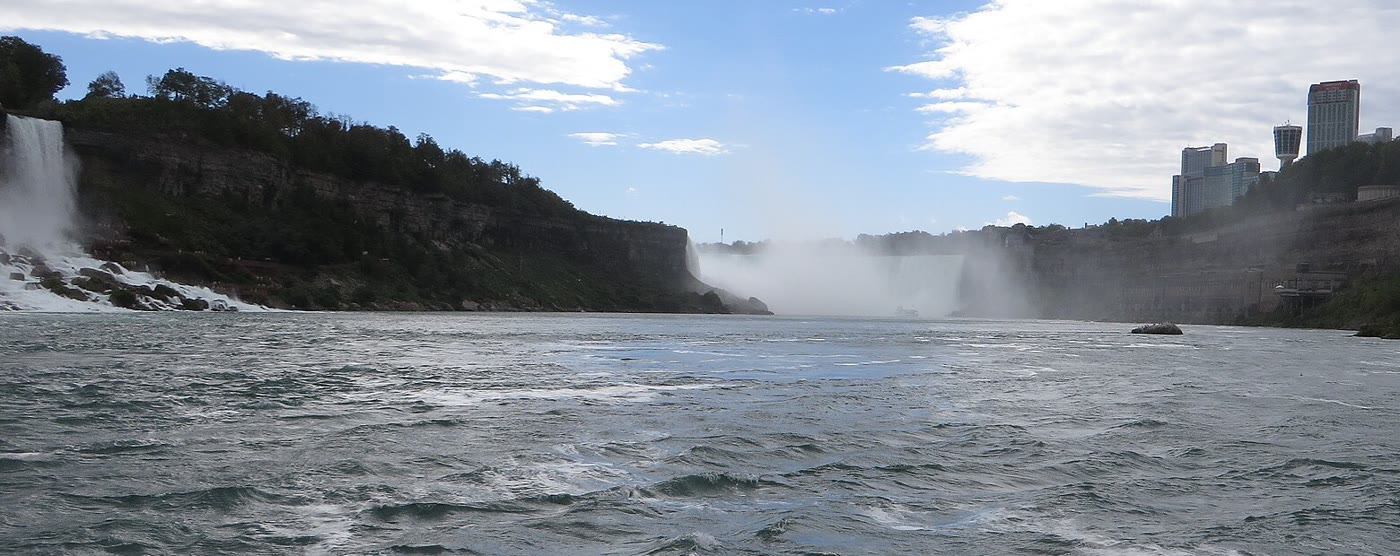
\includegraphics[width=\linewidth]{images/book5/b3-niagara-gorge.jpg}

{\scriptsize وادي نياغارا، ناظرًا نحو المنبع إلى شلالات الحدوة في ضبابها،
وشلالات أمريكا عند الحافة اليسرى. الصورة:
\mbox{\textdir TLT Ken Lund, CC BY-SA 2.0} (مقتطعة).}
\end{minipage}
\end{inthefield}
% ledger: ijc18:niagara, photo:b3-niagara-gorge


\section{التعرية الجليدية}\label{sec:b3:quantitative-geomorphology:glacial}

ينزلق النهر الجليدي فوق قاعه (الانزلاق القاعدي،
الفصل~\ref{ch:b3:glaciology}) فيعرّيه بالكشط، إذ تكشط الفتات المحمولة في الجليد الصخرَ،
وبالاقتلاع، إذ يسحب كتلًا فكّكتها
الشقوق. ويتناسب الاثنان مع سرعة الانزلاق.

\begin{definition}[قانون التعرية الجليدية]\label{def:b3:quantitative-geomorphology:glacial}
\emph{قانون التعرية الجليدية}\index{قانون التعرية الجليدية} يعطي معدّل تعرية قاع النهر الجليدي
بالصيغة $E = K_G\,u_s^{\,l}$، حيث $u_s$ هي
سرعة الانزلاق، و$K_G$ معامل، و$l$ أسّ.
\end{definition}

تأخذ نماذج المناظر عادةً $l = 1$، مع استعمال قيم بين 1 و2.
جمعت دراسةٌ شملت 38 نهرًا جليديًا، تمتدّ معدّلات تعريتها عبر
خمس رتب من القدر، فوجدت أنّ التعرية مرتبطة بسرعة الانزلاق، مع $l = 0.65$
و$K_G = 10^{-4}$ عندما تُقاس $E$ بالمتر في السنة: تكون التعرية أسرع تحت الأنهار الجليدية المعتدلة
التي تغذّيها الثلوج الوفيرة، وهي التي تنزلق بسرعة. ولأنّ الجليد أسمك
وأسرع ما يكون على محور الوادي، يتعمّق القاع أكثر من
الجانبين، فيأخذ الوادي شكل حرف U.
% ledger: cook20:glacial

\begin{definition}[المنشار الجليدي]\label{def:b3:quantitative-geomorphology:buzzsaw}
\emph{المنشار الجليدي}\index{المنشار الجليدي} هو الحدّ الذي تفرضه الأنهار الجليدية على
ارتفاع السلسلة الجبلية: حيث يعلو الصخر على الارتفاع
الذي تتكوّن عنده الأنهار الجليدية، تعريه بالسرعة نفسها التي يرتفع بها، أيًّا كان
معدّل الرفع، فتتجمّع القمم ومتوسط الارتفاع قرب ذلك الارتفاع.
\end{definition}

\section{التكتونية والتعرية}\label{sec:b3:quantitative-geomorphology:tectonics}

\begin{definition}[الحالة المستقرّة الطبوغرافية]\label{def:b3:quantitative-geomorphology:steady-state}
يكون المشهد الطبيعي في \emph{الحالة المستقرّة الطبوغرافية}\index{الحالة المستقرّة الطبوغرافية}
حين يتساوى معدّل تعريته مع معدّل رفع الصخر في كلّ مكان، بحيث
لا تتغيّر ارتفاعاته رغم مرور الصخر عبره.
\end{definition}

تختبر المعدّلات المقاسة عبر فترات زمنية مختلفة هذه الحالة. تعطي النويدات
الكونية المنشأ في رمل الأنهار متوسطَ معدّل تعرية الحوض خلال الزمن
اللازم لإزالة طبقة بحدود طول توهين إنتاجها،
أي نحو \qty{55}{cm} من الصخر؛ أمّا الميقاتيات الحرارية وعلاقات العمر بالارتفاع فتعطي
معدّل الاستخراج عبر ملايين السنين. وحين تتفق الاثنتان مع بعضهما
ومع معدّل الرفع، يُرجَّح أنّ المشهد الطبيعي في \omterm{def:b3:quantitative-geomorphology:steady-profile}{الحالة المستقرّة}؛ وحين
يكون المعدّل قصير المدى أسرع في المجاري الدنيا منه في المنابع،
فذلك دليل على مرور نقطة انقطاع. كما أنّ إزالة الصخر تخفّف الحمل عن
الغلاف الصخري، فيرتفع استجابةً لذلك.
% ledger: zech04:exposure

\begin{definition}[الارتداد الأيزوستاتي الحتّي]\label{def:b3:quantitative-geomorphology:rebound}
\emph{الارتداد الأيزوستاتي الحتّي}\index{الارتداد الأيزوستاتي الحتّي} هو
ارتفاع سطح الصخر في منطقة في توازن أيزوستاتي،
استجابةً للكتلة التي تزيلها التعرية.
\end{definition}

\begin{proposition}[ترتفع القمم حين تتعمّق الأودية]\label{prop:b3:quantitative-geomorphology:rebound}
في التوازن الأيزوستاتي لآيري، حين تكون القشرة كثافتها $\rho_c$ فوق وشاح كثافته $\rho_m$،
فإنّ إزالة سماكة متوسطة $\bar e$ من القشرة عن منطقة ما ترفع المنطقة
كلّها بمقدار $(\rho_c/\rho_m)\,\bar e$. وإذا اقتصرت التعرية
على الأودية، فإنّ القمم غير المتعرّضة ترتفع بذلك المقدار، بينما
ينخفض متوسط السطح بمقدار $(1 - \rho_c/\rho_m)\,\bar e$ فقط.
\end{proposition}

\begin{proof}
يقتضي التعويض أن تبقى كتلة كلّ عمود فوق عمق ثابت
كما هي. إزالة سماكة $\bar e$ من القشرة، متوسطةً على مساحة
التعويض، تُخفض الكتلة لكلّ وحدة مساحة بمقدار $\rho_c \bar e$؛
ولتعويضها يلزم أن يتدفّق الوشاح إلى الأعماق، فيرفع قاعدة العمود،
وكلّ ما عليه، بمقدار $\delta$ حيث $\rho_m \delta = \rho_c \bar
e$. ترتفع القمّة التي لم تفقد صخرًا بمقدار $\delta$؛ ويفقد متوسط السطح
$\bar e$ ويكتسب $\delta$.
\end{proof}

تبلغ الكثافة المرجّحة بالسماكة لقشرة نموذج الأرض المرجعي
\qty{2.72}{g/cm^3} وكثافة الوشاح تحت الموهو \qty{3.38}{g/cm^3}،
بنسبة 0.80: فمن كلّ مئة متر من الصخر المتعرّض يخسر متوسط السطح
عشرين مترًا فقط. ولذلك يمكن للحفر العميق لهضبة قديمة أن يرفع قممها
حتى وهي تتآكل.
% ledger: prem:crust-mantle-ratio

\begin{omfigure}
\begin{tikzpicture}[x=0.6cm, y=0.6cm, font=\scriptsize]
\begin{scope}
\fill[omDef!12] (0,0) rectangle (8,4);
\draw[thick] (0,4) -- (8,4);
\draw[densely dashed] (0,0) -- (8,0);
\node[anchor=north] at (4,-0.1) {قاعدة القشرة};
\node at (4,2) {\foreignlanguage{arabic}{القشرة $\rho_c$}};
\node at (4,-1.2) {\foreignlanguage{arabic}{الوشاح $\rho_m$}};
\node[anchor=south] at (4,4.1) {قبل};
\end{scope}
\begin{scope}[xshift=6.2cm]
\fill[omDef!12] (0,0.8) -- (0,4.8) -- (1.4,4.8) -- (2.0,2.4) -- (2.6,4.8) -- (5.4,4.8) -- (6.0,2.4) -- (6.6,4.8) -- (8,4.8) -- (8,0.8) -- cycle;
\draw[thick] (0,4.8) -- (1.4,4.8) -- (2.0,2.4) -- (2.6,4.8) -- (5.4,4.8) -- (6.0,2.4) -- (6.6,4.8) -- (8,4.8);
\draw[black!50, densely dashed] (0,4) -- (8,4);
\draw[densely dashed] (0,0.8) -- (8,0.8);
\draw[densely dashed, black!40] (0,0) -- (8,0);
\draw[<->, omThm] (8.3,4.05) -- (8.3,4.75) node[midway, right] {$\delta$};
\draw[<->, omThm] (8.3,0.05) -- (8.3,0.75) node[midway, right] {$\delta$};
\node[anchor=west, font=\scriptsize] at (8.1,2.4) {$\delta = (\rho_c/\rho_m)\,\bar e$};
\node[anchor=south] at (4,5.0) {بعد الحفر الرأسي للأودية};
\node[anchor=north] at (2.0,2.3) {واد};
\end{scope}
\end{tikzpicture}

\par\smallskip{\small \omterm{def:b3:quantitative-geomorphology:rebound}{الارتداد الأيزوستاتي الحتّي}، تخطيطيًّا. يؤدّي قطع
الأودية إلى إزالة سمك متوسّط $\bar e$ من القشرة؛ فيرتفع العمود بمقدار
$\delta = (\rho_c/\rho_m)\bar e$ عند قاعدته وعند قممه غير المتأثّرة
(الخطّ الرمادي المتقطّع هو السطح القديم).}\label{fig:b3:quantitative-geomorphology:rebound}
\end{omfigure}

\section{التمارين}

\begin{exercise}[$\star$]\label{exo:b3:quantitative-geomorphology:1}
جرف خط الشاطئ بإزاحة \qty{4}{m} ($a = \qty{2}{m}$) يقع على منحدر
الحقل البعيد البالغ 0.04، وبلغ أشدّ انحدار له الآن 0.30. احسب
$\kappa t$، ثم عمر الجرف عند $\kappa = \qty{5e-3}{m^2/yr}$.
\end{exercise}
% ledger: whipple04:scarp-erf, whipple04:scarp-kappa

\begin{exercise}[$\star$]\label{exo:b3:quantitative-geomorphology:2}
يعطي مسح الليدار تقوّس قمّة تلّة قدره \qty{-0.012}{m^{-1}} على ظهرة
معامل انتشارها \qty{4e-3}{m^2/yr}. احسب معدّل تعريتها بوحدة
\unit{mm/yr}، وفرق التضاريس بين قمّتها والقنوات
الواقعة على بعد \qty{80}{m}، بافتراض \omterm{def:b3:quantitative-geomorphology:steady-profile}{الحالة المستقرّة}.
\end{exercise}

\begin{exercise}[$\star$]\label{exo:b3:quantitative-geomorphology:3}
مع $m = 0.5$، و$n = 1$، و$K = \qty{2e-6}{yr^{-1}}$، احسب معدّل
الحفر الرأسي لنهر يصرّف \qty{25}{km^2} على انحدار 0.01.
ما وحدات $K$ من أجل قيم عامّة للمعاملين $m$ و$n$؟
\end{exercise}

\begin{exercise}[$\star$]\label{exo:b3:quantitative-geomorphology:4}
تُظهر ثلاثة أنهار نقاط انقطاع: (أ) حيث تقطع طبقةُ الحجر الرملي واديًا
محفورًا في الطَّفل؛ (ب) حيث يعبر نهر صدعًا عاديًّا نشطًا من
الجدار المرتكز إلى الجدار المعلّق؛ (ج) في كلّ نهر من أنهار حوض، كلّها
عند الارتفاع نفسه تقريبًا، على بعد بضعة كيلومترات من ساحل ارتفع في
زلزال. أيّها ثابت وأيّها سيتنقّل؟
\end{exercise}

\begin{exercise}[$\star\star$]\label{exo:b3:quantitative-geomorphology:5}
من أجل $m = 1$ و$n = 2$، احسب $\theta$ والانحدار المستقرّ حيث $A =
\qty{10}{km^2}$، مع $U = \qty{0.1}{mm/yr}$ و$K = 10^{-9}$ بوحدتي
المتر والسنة.
بأيّ عامل يتغيّر مؤشّر الانحدار إذا تضاعف $U$؟ قارن مع $n =
1$.
\end{exercise}

\begin{exercise}[$\star\star$]\label{exo:b3:quantitative-geomorphology:6}
تنمو مساحة تصريف النهر مع المسافة $d$ عن خطّ تقسيمه المائي وفق $A =
c\,d^{h}$. أثبت أنّه، مقيسًا صعودًا من مصبّه عند $d = L$،
\[
\chi(d) = \frac{A_0^{\theta}}{c^{\theta}}\,\frac{L^{p} - d^{p}}{p},
\qquad p = 1 - h\theta ,
\]
واحسبه من أجل $c = 2$ \babelsublr{(SI)}، و$h = 1.8$، و$\theta = 0.45$، و$A_0 =
\qty{1}{km^2}$، و$L = \qty{20}{km}$، و$d = \qty{5}{km}$.
\end{exercise}

\begin{exercise}[$\star\star$]\label{exo:b3:quantitative-geomorphology:7}
مع $n = 1$، و$m = 0.5$، و$K = \qty{2e-6}{yr^{-1}}$، احسب
سرعة تقدّم نقطة انقطاع حيث $A = \qty{100}{km^2}$، بوحدة m/kyr، والزمن
اللازم لقطع \qty{5}{km} بتلك السرعة. لماذا يستغرق
فعلًا وقتًا أطول؟
\end{exercise}

\begin{exercise}[$\star\star$]\label{exo:b3:quantitative-geomorphology:8}
أودية عمقها \qty{600}{m}، تشغل في المتوسّط \qty{40}{\percent} من
مساحة هضبة، وتُحفر فيها. مع $\rho_c/\rho_m = 0.80$، احسب
متوسّط السمك المتعرّى، وارتفاع القمم، والتغيّر في متوسّط
الارتفاع.
\end{exercise}
% ledger: prem:crust-mantle-ratio

\begin{exercise}[$\star\star$]\label{exo:b3:quantitative-geomorphology:9}
لدينا \omterm{def:b3:quantitative-geomorphology:soil-production}{دالة إنتاج التربة} حيث $P_0 = \qty{0.3}{mm/yr}$ و$h_0 =
\qty{0.5}{m}$. احسب سُمك التربة المستقرّ عند تعرية بمعدّل
\qty{0.05}{mm/yr} وعند \qty{0.2}{mm/yr}. ماذا يحدث عند
\qty{0.4}{mm/yr}؟
\end{exercise}

\begin{exercise}[$\star\star\star$]\label{exo:b3:quantitative-geomorphology:10}
تتعرّى تلّة في \omterm{def:b3:quantitative-geomorphology:steady-profile}{الحالة المستقرّة} بمعدّل $E = \qty{0.1}{mm/yr}$ مع $\kappa =
\qty{5e-3}{m^2/yr}$ وقانون \omterm{def:b3:quantitative-geomorphology:critical}{انحدار السفح الحرج} غير الخطّي، آخذًا
$S_c = 1.2$ لأجل التمرين. أثبت أنّ الدفق عند مسافة $x$ من
تقسيمه المائي يساوي $E x$، أوجد الانحدار، واحسبه عند 20 و50 و100
و\qty{200}{m}. قارن بالانتشار الخطّي، وصِف شكل
التلّة.
\end{exercise}

\begin{exercise}[$\star\star\star$]\label{exo:b3:quantitative-geomorphology:11}
أثبت أنّ زمن استجابة شبكة نهرية لتغيّر عند مصبّها،
من أجل $n = 1$، هو $\chi_h/(K A_0^m)$، حيث $\chi_h$ أكبر قيمة للمقدار
$\chi$ عند رأس القناة. احسبه لنهر المرتفعات الوارد في الأشكال
($A_0 = \qty{1}{km^2}$، $m = 0.5$، $K = \qty{e-6}{yr^{-1}}$)، أوّلًا من أجل
جذعه وحده، الذي رأسه عند $\chi = \qty{5464}{m}$، ثم من أجل الشبكة،
التي أعلى رأس فيها، الواقع على الرافد 1، عند $\chi = \qty{7237}{m}$.
\end{exercise}

\begin{exercise}[$\star\star\star$]\label{exo:b3:quantitative-geomorphology:12}
في شبكة فيها $n = 1$ و$U$ منتظم، يجري رافد واحد على صخر قابل للتعرية ضعفَي
ما عداه ($2K$) فوق ملتقاه، عند $\chi_j$. أثبت أنّ
خطّه المستقرّ في المستوى $(\chi, z)$ يملك نصف ميل الجذع
فوق $\chi_j$، وأنّ نقطة انقطاع نشأت عند المصبّ تبلغ،
عند الزمن الذي تكون فيه نقطة انقطاع الجذع عند $\chi_k > \chi_j$، النقطة
ذات $\chi = \chi_j + 2(\chi_k - \chi_j)$ من ذلك الرافد.
\end{exercise}

\section{مسألة: شلّال نهر فاردن}

\begin{problem}[{مسألة نهاية الأسبوع --- المقطع الطولي ومؤشّر الانحدار وقابلية
التعرية لنهر مرتفعات مُختلَق، وعمر شلّاله}]
\label{pb:b3:quantitative-geomorphology:1}
غرب تلال فاردن، يُصرّف النهر مرتفعات من الشيست قبل أن
يدخل الخريطة عند حافّتها الغربية، على ارتفاع \qty{170}{m}. صعودًا
من تلك النقطة، أي مصبّه، يبلغ طول الجذع \qty{12}{km} من تقسيمه المائي،
وبمساحة تصريف $A = 4.5\,d^{1.7}$ (\unit{m^2}، و$d$ بالمتر من
خطّ التقسيم)، ورأس قناة عند $d = \qty{300}{m}$. خذ معدّل الرفع الصخري
مساويًا لمعدّل التجريد لحوض نهر فاردن المستخلص من حمولاته
في مجلد السنة الأولى، \qty{43}{m/Myr}. وخذ $n = 1$ ومساحة المرجع $A_0 = \qty{1}{km^2}$.
يقع على الجذع شلّال ارتفاعه \qty{25}{m}، على بعد \qty{4.60}{km} صعودًا من
المصبّ. جميع القيم مُختلَقة.

\medskip\noindent\textbf{الجزء الأول --- المقطع الطولي.}
\begin{enumerate}
\item احسب مساحة التصريف عند المصبّ وعند رأس القناة.
\item الانحدارات المقاسة على مقاطع طولها \qty{200}{m}، بعيدًا عن
  الشلّال:

  \smallskip
  {\small\begin{tabular}{l*{6}{c}}
  \mbox{\textdir TLT $A$ (\unit{km^2})} & 0.388 & 0.587 & 0.888 & 1.345 & 2.036 & 3.082 \\
  $S$ & 0.06641 & 0.05026 & 0.04888 & 0.03322 & 0.03688 & 0.02688 \\[2pt]
  \mbox{\textdir TLT $A$ (\unit{km^2})} & 4.665 & 7.061 & 10.69 & 16.18 & 24.49 & 37.08 \\
  $S$ & 0.01921 & 0.01713 & 0.01545 & 0.01419 & 0.007922 & 0.007855
  \end{tabular}}

  \smallskip
  قدّر \omterm{def:b3:quantitative-geomorphology:indices}{مؤشّر التقعّر} من النقطة الأولى والنقطة الأخيرة.
\item ميل المربعات الصغرى للمتغيّر $\log S$ بدلالة $\log A$ يساوي $-0.466$.
  هل يتّفق مع $\theta = 0.5$؟
\item مع $\theta_{\mathrm{ref}} = 0.5$، احسب $k_{sn} = S A^{0.5}$ ($A$ بوحدة
  \unit{m^2}) للنقطتين الأولى والأخيرة، واذكر ماذا يمثّل المتوسّط
  الهندسي للقيم الاثنتي عشرة، البالغ \qty{45.1}{m}.
\item لماذا تتشتّت الانحدارات أكثر بكثير من الارتفاعات؟
\item باستخدام صيغة تمرين \omterm{def:b3:quantitative-geomorphology:chi}{تحليل كاي}، احسب $\chi$ عند $d =
  \qty{9.00}{km}$، نقطة تقع أسفل الشلّال.
\end{enumerate}

\medskip\noindent\textbf{الجزء الثاني --- الانحدار وقابلية التعرية.}
\begin{enumerate}[resume]
\item يقع النهر على ارتفاع \qty{193.4}{m} عند $d = \qty{9.00}{km}$. احسب
  ميل مخطّط كاي أسفل الشلّال \omterm{def:b3:quantitative-geomorphology:indices}{ومؤشّر انحدار القناة} $k_{sn}$.
\item أيّ التقديرين للمؤشّر $k_{sn}$، هذا أم تقدير المساحة والانحدار،
  تثق به أكثر، ولماذا؟
\item بافتراض \omterm{def:b3:quantitative-geomorphology:steady-profile}{الحالة المستقرّة} أسفل الشلّال، احسب $K$ انطلاقًا من
  معدّل الرفع.
\item تحقّق من أنّ معدّل الحفر الرأسي عند المصبّ، الذي انحداره
  0.00691، يساوي معدّل الرفع.
\item احسب سرعة تقدّم \omterm{def:b3:quantitative-geomorphology:knickpoint}{نقطة الانقطاع} عند المصبّ وعند
  الشلّال، بوحدة m/kyr.
\item احسب ارتفاع رأس القناة على المقطع الطولي المستقرّ،
  وتضاريس الجذع.
\end{enumerate}

\medskip\noindent\textbf{الجزء الثالث --- الشلّال.}
\begin{enumerate}[resume]
\item لماذا حافظ الشلّال، مع $n = 1$، على ارتفاع سقوط
  \omterm{def:b3:quantitative-geomorphology:knickpoint}{مستوى القاعدة}؟
\item احسب $\chi$ عند الشلّال.
\item احسب الزمن الذي استغرقته \omterm{def:b3:quantitative-geomorphology:knickpoint}{نقطة الانقطاع} من المصبّ حتى موضعها
  الحالي.
\item أين ستكون بعد \qty{300}{kyr} من الآن؟
\item ينضمّ الرافد 3 إلى الجذع على بعد \qty{2.5}{km} صعودًا من المصبّ؛ ويبلغ
  طوله \qty{5}{km}، وبمساحة تصريف $A = 1.5\,s^{1.7}$ ($s$ من خطّ تقسيمه الخاص).
  أين ينبغي أن يقع شلّاله؟
\item ينضمّ الرافدان 1 و2 إلى الجذع على بعد 8 و\qty{5}{km} صعودًا من
  المصبّ. اشرح لماذا لا يوجد لهما شلّال.
\end{enumerate}

\medskip\noindent\textbf{الجزء الرابع --- السفوح والعمر.}
\begin{enumerate}[resume]
\item يعطي مسح بالليدار فوق الشلّال انحناءً لقمّة التلّ مقداره
  \qty{-0.0086}{m^{-1}}. مع $\kappa = \qty{5e-3}{m^2/yr}$، احسب
  معدّل التعرية، وقارنه بمعدّل الرفع.
\item تبلغ أطوال السفوح نحو \qty{150}{m}. قارن زمن استجابتها
  $L^2/\kappa$ بالعمر الذي وُجد في الجزء الثالث.
\item صف السفوح أسفل الشلّال اليوم، وكيف
  ستتغيّر.
\item معدّل الرفع معلوم بدقّة \qty{20}{\percent}. أعطِ مدى
  العمر.
\item كيف كان سيتطوّر الشلّال لو كانت $n$ تساوي 2؟
\item أعطِ عمر سقوط \omterm{def:b3:quantitative-geomorphology:knickpoint}{مستوى القاعدة}.
\end{enumerate}
\end{problem}
% ledger: whipple04:steepness, whipple04:scarp-kappa
